\pdfoutput=1
\documentclass[10pt]{beamer}

%STANDARD PREAMBLE
%https://tex.stackexchange.com/questions/68821/is-it-possible-to-create-a-latex-preamble-header
\usepackage{../../rsrc/beamer_preamble}

%% ALLOW FOR ITEMIZE ENVIRONMENTS WITH NO PRECEDING
% SPACING, IF DESIRED
% Reference: https://tex.stackexchange.com/questions/86054/how-to-remove-the-whitespace-before-itemize-enumerate
%\usepackage{enumitem}% http://ctan.org/pkg/enumitem 
\usepackage{paralist}

% RANDOM VARIABLE
\newcommand{\x}{X}
\newcommand{\y}{Y}


\title{Bayesian Inference}

\begin{document}

\maketitle



%\section{Bayesian Approaches}

\begin{frame}{Bayesian approaches}

\begin{itemize}
\item Typically contrasted with \textbf{frequentist} approaches
\item Treat parameters as uncertain, data as fixed
\end{itemize}
\end{frame}

%%%%%%%%%%%%%%

\begin{frame}{Bayes' Rule}
\footnotesize

\begin{sblock}{Bayes' Rule}
$ p(\theta | x) = \dfrac{p(x | \theta) p(\theta)}{p(x)} =\dfrac{p(x | \theta) p(\theta)}{\int p(x | \theta) p(\theta) \, d\theta}  $
\end{sblock}

\begin{sblock}{Terms}

$ \underset{posterior}{p(\theta|x)} = \df{ \underset{likelihood}{p(x|\theta)} \quad  \underset{prior}{p(\theta)} }{ \underset{evidence}{p(x)}} $
\end{sblock}

\begin{sblock}{Posterior}
The posterior distribution is proportional to the prior times the likelihood:
$p(\theta | x) \propto p(x | \theta) p(\theta)$

The posterior distribution \textit{is a distribution} over $\theta$.

\end{sblock}

\begin{sblock}{Evidence}
The evidence, or \textit{marginal likelihood}, can be used for model comparison.
\end{sblock}

\end{frame}

%%%%%

\begin{frame}{Simple Motivation: Batting Averages}

Let 
\begin{itemize}
\item $x$ be observed data (batting average after $n$ at bats)
\item  $\theta$ be parameters (a player's `true` batting average)
\end{itemize}

	\begin{tikzpicture}
  \node (img)  {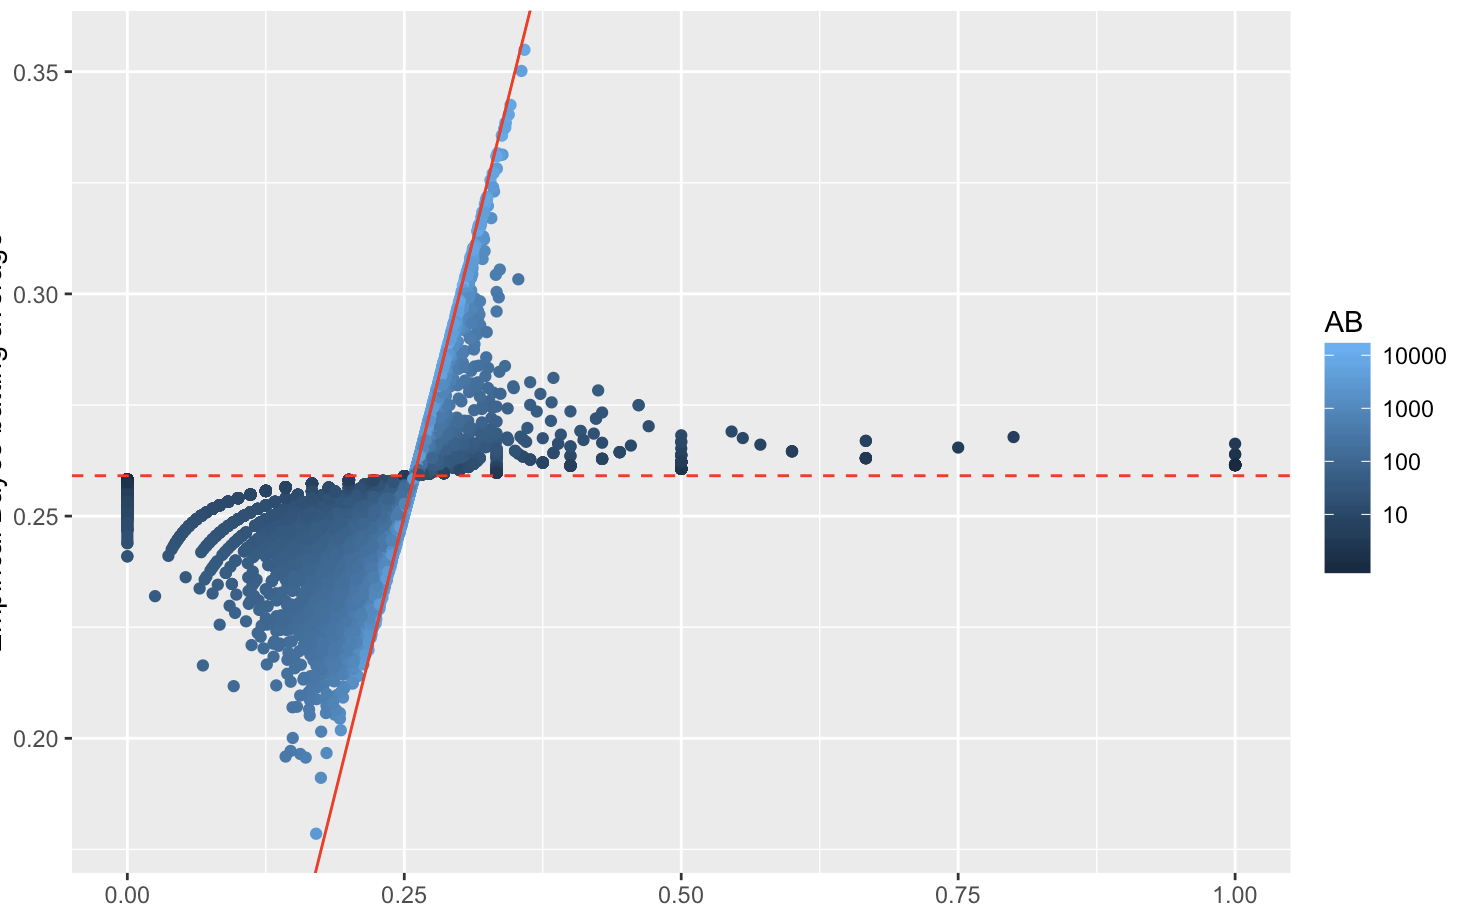
\includegraphics[width=.80\textwidth]{images/batting_averages}} ;
  \node[below=of img, node distance=0cm, yshift=1cm,font=\color{blue}] {Observed data ($x$)};
  \node[left=of img, node distance=0cm, rotate=90, anchor=center,yshift=-0.7cm,font=\color{blue}] {$\E [p (\theta \cond X)]$}; % ($\E_{p(\theta | x)} [\theta]$)};
 \end{tikzpicture}
 


\end{frame}


\begin{frame}{Bayesian Occam's Razor}
\scriptsize

Maximum Likelihood (ML)  solutions tend to overfit.  Bayesian marginalization reduces overfitting.

%\begin{center}
%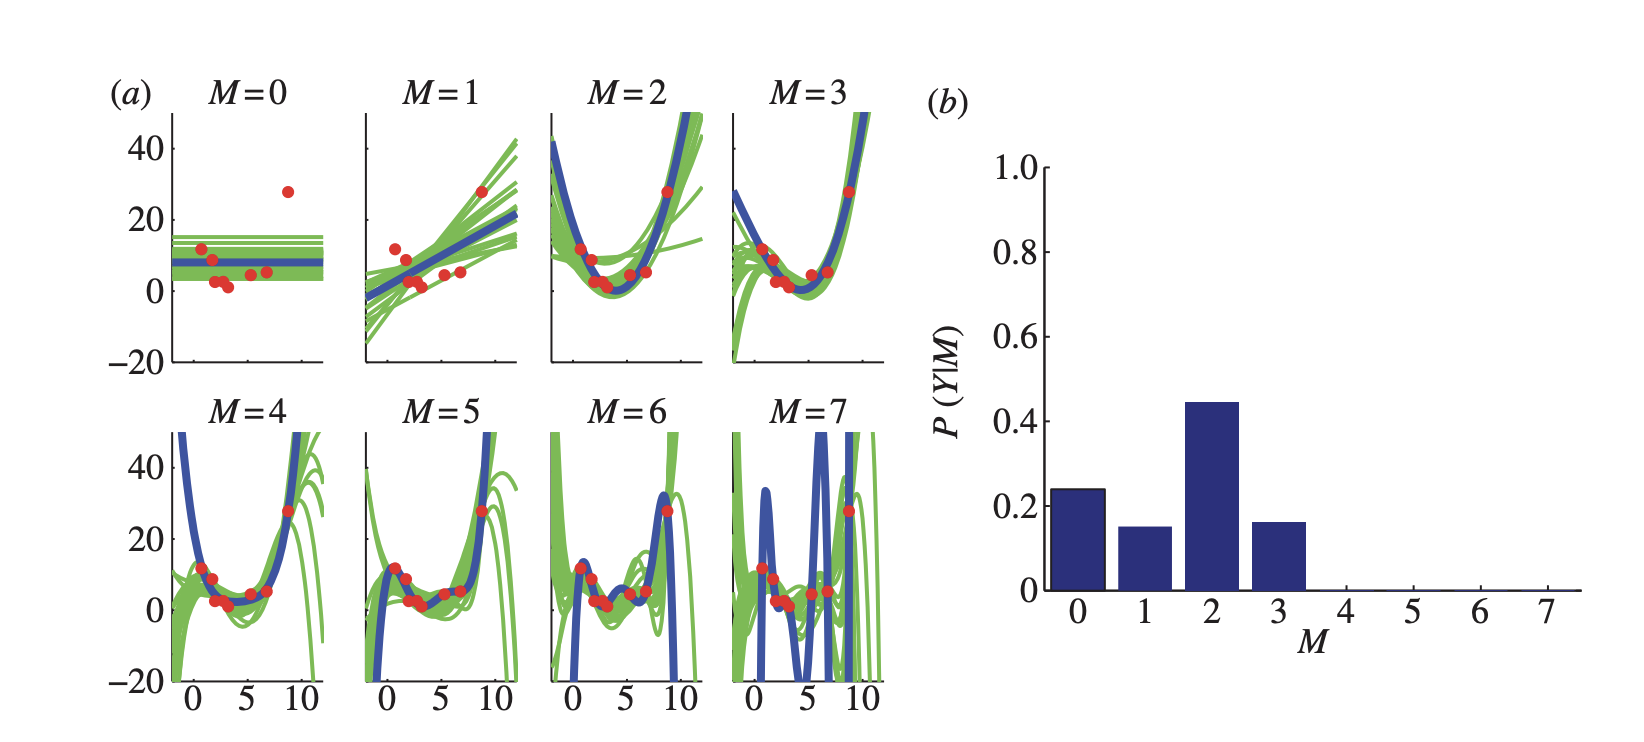
\includegraphics[width=.7\textwidth]{images/occams_razor}
%\end{center}

\begin{minipage}[t]{.47\textwidth}
\begin{center}
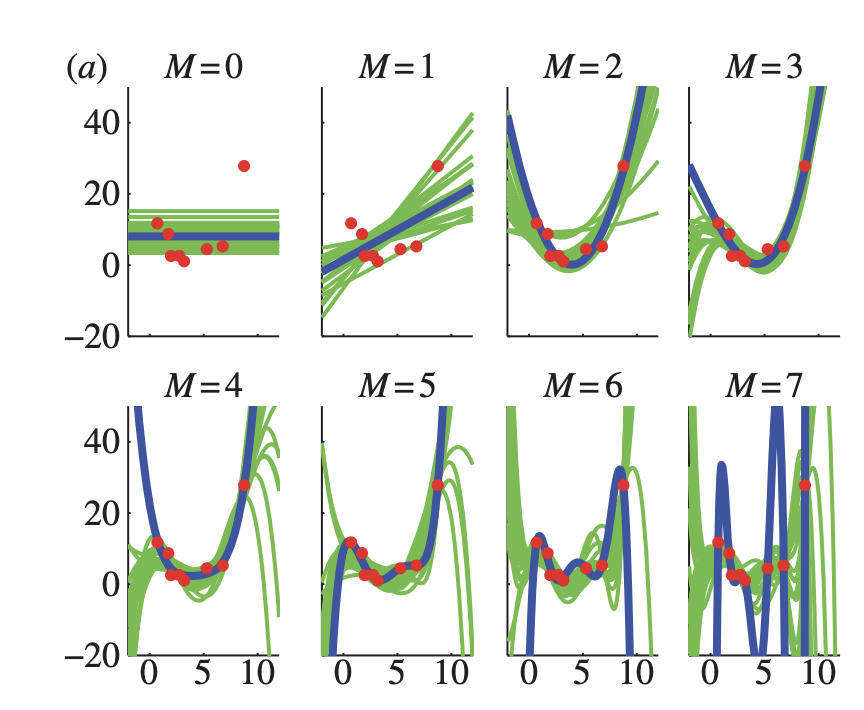
\includegraphics[width=.7\textwidth]{images/occams_razor_a}
\end{center}

Models $y = f(x) + \epsilon$ of  various complexity  \tiny (polynomials of various order, $M$) \scriptsize were fit to 8 data points. 
	\begin{itemize}
	\scriptsize
	\item  Plotted are  \blue{ML} polynomials \tiny (least squares fits to the data under Gaussian noise) \scriptsize and \darkgreen{posterior samples} from a Bayesian model \tiny (which used a Gaussian prior for the coefficients, and an inverse gamma prior on the noise). \scriptsize
	\item The ML estimate can look very different from a typical sample from the posterior!  
	\end{itemize}
\end{minipage}
\hfill
\begin{minipage}[t]{.47\textwidth}
\begin{center}
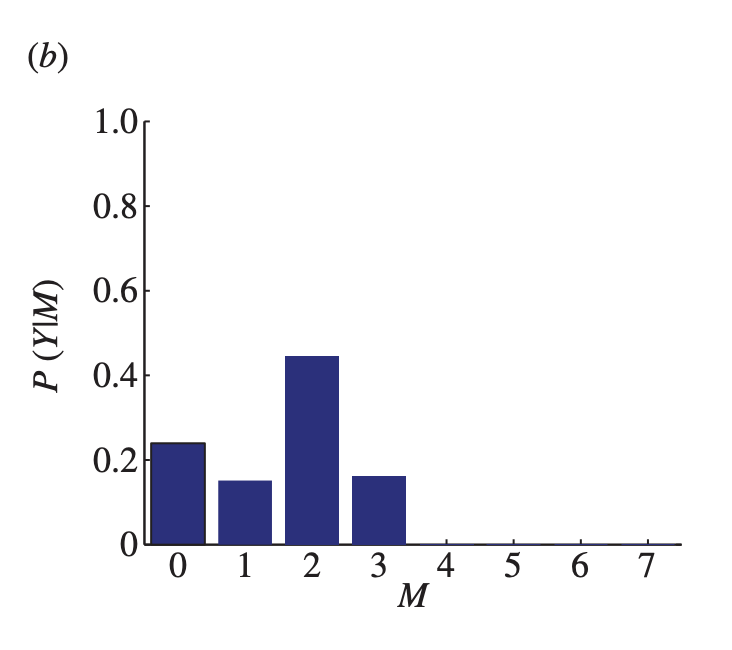
\includegraphics[width=.7\textwidth]{images/occams_razor_b}
\end{center}
The evidence is plotted as a function of model order.  Model orders M=0 to M=3 have considerably higher evidence than other model orders.  We see that Bayesian marginalization has reduced overfitting.  (The maximum likelihood model, the $M=7$ model, fits the data perfectly, but overfits wildly, predicting the function will shoot up or down between neighboring data points.) 
\end{minipage}
\vfill

\hfill \tiny Ghahramani, Z. (2013). Bayesian non-parametrics and the probabilistic approach to modelling. Philosophical Transactions of the Royal Society A: Mathematical, Physical and Engineering Sciences, 371(1984), 20110553.
\end{frame}


%%%%%%%%%%%%%%

\begin{frame}{Posterior predictive distribution}

\begin{sblock}{Given}

$p(\theta | x)$ - posterior \\
$p(\theta)$ - prior \\
$p(x | \theta)$ - likelihood

\end{sblock}

\begin{sblock}{Posterior predictive distribution}

Consider the probability of new data $x'$. Posterior predictive distribution is:

$p(x' | x) = \int p(x', \theta | x) \, d\theta = \int p(x' | \theta, x) p(\theta |x) \, d\theta = \int p(x' | \theta) p(\theta | x) \, d\theta$

Incorporates the knowledge and uncertainty about $\theta$ that we still had after seeing data $x$.

\end{sblock}

\end{frame}

%%%%%%%%%



%%%%%%%%%

\begin{frame}{Bayesian inference: conjugate example}
Sometimes, we can compute the posterior distribution by hand, given prior and likelihood.

\begin{sblock}{Setup: flipping a coin}
Probability that it lands heads is (unknown) $\theta$. \\
Prior probability over $\theta$ assumed to follow a $Beta(3,3)$ distribution:
$$ p(\theta) = \frac{\theta^{3-1}(1-\theta)^{3-1}}{B(3,3)}$$
Note: $\theta \sim Beta(a, b)$ means $p(\theta) \propto \theta^{a-1}(1-\theta)^{b-1}$\\
Will collect data by flipping coin once. Likelihood of observing heads ($x=1$) or tails ($x=0$) is given by a Bernoulli distribution:
$$p(x | \theta) = \theta^x(1-\theta)^{1-x} $$.
\end{sblock}


\end{frame}

\begin{frame}{Bayesian inference: conjugate example}

\begin{sblock}{Setup: flipping a coin}
Probability that it lands heads is (unknown) $\theta$. \\
Prior probability over $\theta$ assumed to follow a $Beta(3,3)$ distribution:
$$ p(\theta) = \frac{\theta^{3-1}(1-\theta)^{3-1}}{B(3,3)}$$
Note: $\theta \sim Beta(a, b)$ means $p(\theta) \propto \theta^{a-1}(1-\theta)^{b-1}$\\
Will collect data by flipping coin once. Likelihood of observing heads ($x=1$) or tails ($x=0$) is given by a Bernoulli distribution:
$$p(x | \theta) = \theta^x(1-\theta)^{1-x} $$.
\end{sblock}
\begin{sblock}{Computing the posterior after observing x=1}
$$p(\theta| x) \propto p(x | \theta) p(\theta) = \theta^1(1-\theta)^{0}  \theta^{2}(1-\theta)^{2}  = \theta^3 (1-\theta)^2 \implies \theta | x \sim Beta(4,3)$$
\end{sblock}

\end{frame}

%%%%%%%%%%%%%%%

\begin{frame}{Bayesian inference: tractability notes}

\begin{sblock}{Conjugacy}
We have conjugacy when the prior and the posterior distributions are in the same family (e.g. in the previous example, the prior and posterior are beta distributions).
\end{sblock}

\begin{sblock}{Generally}
Generally, computing the posterior distribution is much harder than in this example!
\vfill
Consider the denominator in $ p(\theta | x) = \dfrac{p(x | \theta) p(\theta)}{\int p(x | \theta) p(\theta)} \, d\theta $  - integrals are hard 
\vfill
In nonconjugate examples, we need approaches to work with the posterior distribution when we cannot calculate it directly. Stay tuned!
\end{sblock}

\end{frame}




%%%%%%%%%%%%%%%%







\end{document}